\documentclass{article}

\usepackage{graphicx}
\usepackage{tikz}
\usepackage{tikzsymbols}
\usetikzlibrary{calc,patterns,shapes.geometric}
\pagestyle{empty}
\usepackage[margin=0pt]{geometry}
\geometry{papersize={14in,12in}}

\def\centerarc[#1](#2)(#3:#4:#5){\draw[#1] ($(#2)+({#5*cos(#3)},{#5*sin(#3)})$) arc (#3:#4:#5);}

\begin{document}
	\begin{figure}
		\centering
		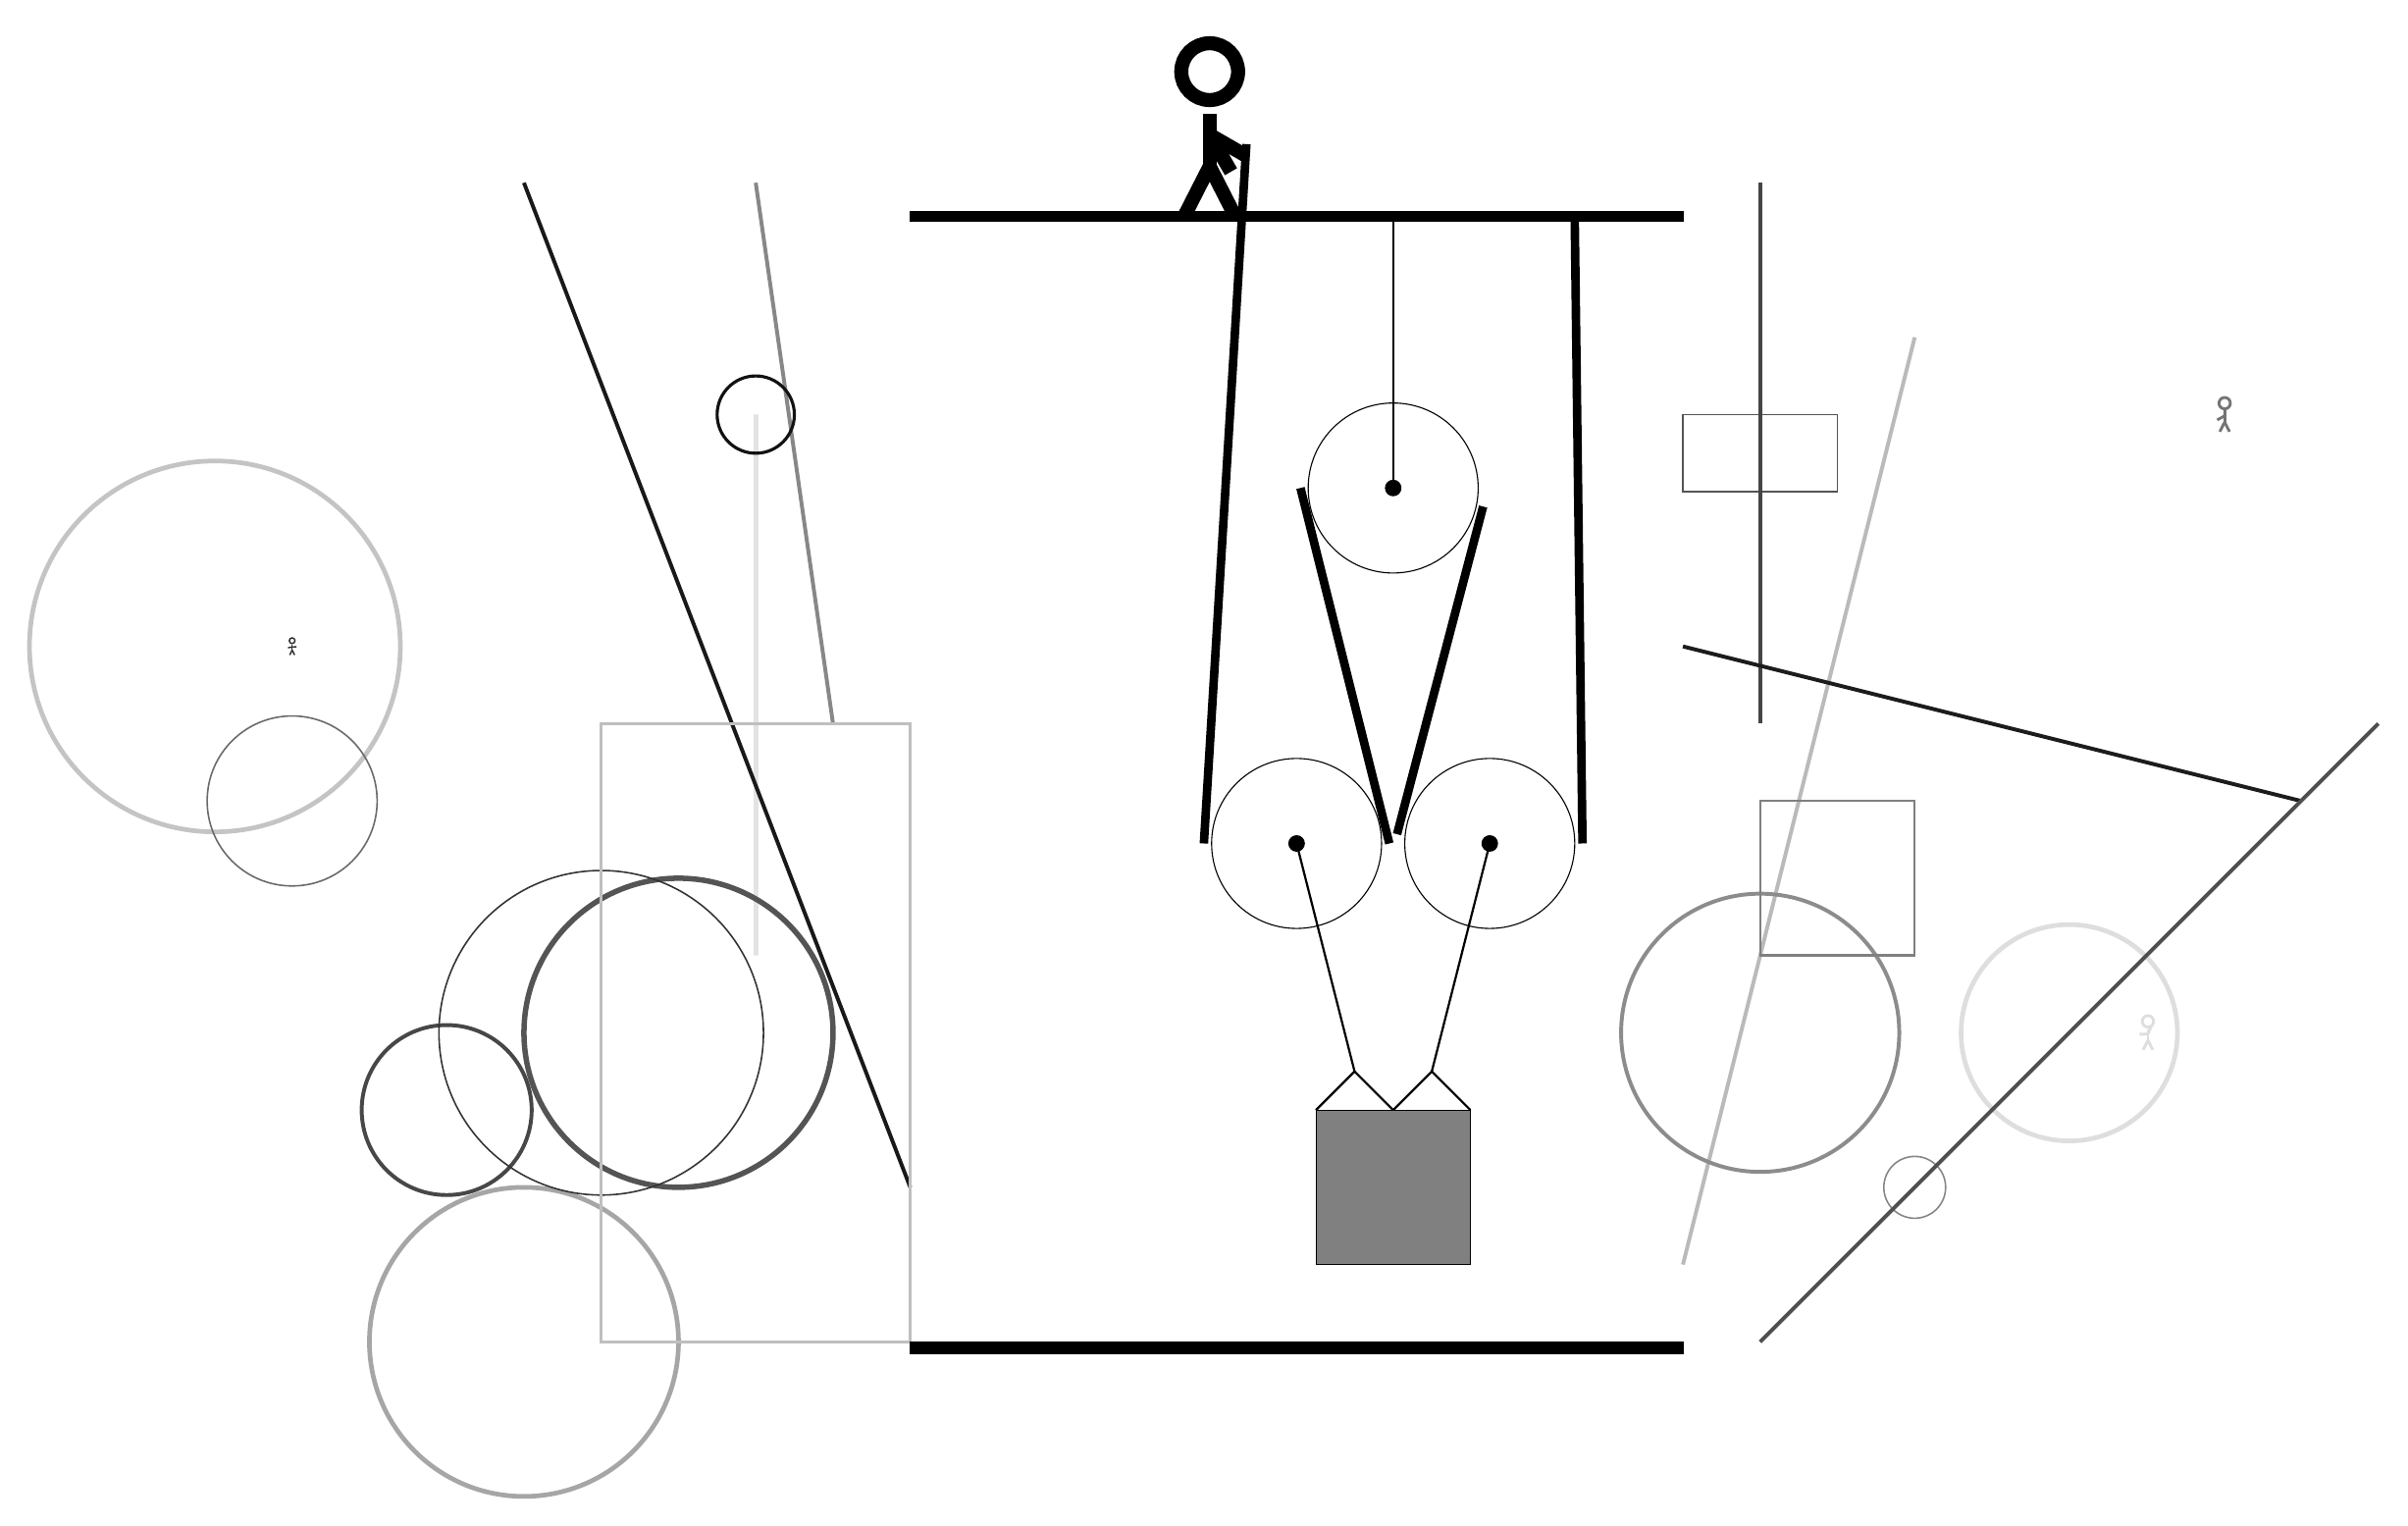
\begin{tikzpicture}
			%%%%% START %%%%%
			
			\draw[fill=black] (-4, 11.5) rectangle (6, 11.625);
			
			\draw (1, 3.45) circle (1.1);
			\draw[fill=black] (1, 3.45) circle (0.1);
			
			\draw[line width=0.6mm, color=black!11] (-6, 9) rectangle (-6, 2);
			
			\draw[line width=0.5mm, color=black!74] (6, 8) rectangle (6, 8);
			\draw[line width=0.5mm, color=black!47](-6, 12) -- (-5, 5);
			\draw[line width=0.5mm, color=black!27](9, 10) -- (6, -2);
			\draw [line width=0.5mm, color=black!72](-10, 0) circle (1.1);
			\draw [line width=0.5mm, color=black!45](7, 1) circle (1.8);
			\draw [line width=0.7mm, color=black!67](-7, 1) circle (2.0);
			
			\draw[line width=0.2mm, color=black!67] (8, 9) rectangle (6, 8);
			\node[line width=0.3mm, color=black!83] at (-12, 6) {\Strichmaxerl[1][10][3]};
			
			\draw [line width=0.6mm, color=black!13](11, 1) circle (1.4);
			\draw[line width=0.5mm, color=black!73](7, 12) -- (7, 5);
			\draw [line width=0.6mm, color=black!23](-13, 6) circle (2.4);
			\node[line width=0.5mm, color=black!54] at (13, 9) {\Strichmaxerl[2][29][87]};
			\draw [line width=0.6mm, color=black!35](-9, -3) circle (2.0);
			\draw[line width=0.3mm, color=black!50] (7, 4) rectangle (9, 2);
			\draw[line width=0.5mm, color=black!89](6, 6) -- (14, 4);
			\draw [line width=0.2mm, color=black!48](9, -1) circle (0.4);
			\node[line width=0.2mm, color=black!13] at (12, 1) {\Strichmaxerl[2][2][67]};
			\draw[line width=0.5mm, color=black!69](7, -3) -- (15, 5);
			
			\draw [line width=0.2mm, color=black!59](-12, 4) circle (1.1);
			\draw [line width=0.2mm, color=black!80](-8, 1) circle (2.1);
			\draw[line width=0.5mm, color=black!90](-9, 12) -- (-4, -1);
			
			\draw [line width=0.4mm, color=black!93](-6, 9) circle (0.5);
			\draw[line width=0.4mm, color=black!25] (-4, 5) rectangle (-8, -3);
			
			\draw (2.25, 8.05) circle (1.1);
			\draw[fill=black] (2.25, 8.05) circle (0.1);
			\draw[thick] (2.25, 8.05) -- (2.25, 11.5);
			
			\draw (3.5, 3.45) circle (1.1);
			\draw[fill=black] (3.5, 3.45) circle (0.1);
			
			\draw[thick] (3.5, 3.45) -- (2.75, 0.5);
			\draw[thick] (1, 3.45) -- (1.75, 0.5);
			\draw[thick]  (1.25, 0) -- (1.75, 0.5) -- (2.25, 0);
			\draw[thick]  (2.25, 0) -- (2.75, 0.5) -- (3.25, 0);
			\draw[fill=black!50] (1.25, 0) rectangle (3.25, -2);
			
			\draw[line width=1.1mm] (0.35, 12.5) --  (-0.2, 3.45);
			\centerarc[line width=1.1mm](1, 3.45)(180:360:1.2000000000000002);
			\draw[line width=1.1mm] (2.2, 3.45) -- (1.05, 8.05);
			\centerarc[line width=1.1mm](2.25, 8.05)(-20:180:1.2000000000000002);
			\draw[line width=1.1mm](3.414, 7.81) -- (2.3, 3.57);
			\centerarc[line width=1.1mm](3.5, 3.45)(160:360:1.2000000000000002);
			\draw[line width=1.1mm](4.7, 3.45) -- (4.6, 11.5);
			
			\node at (-0.07, 12.7) {\Strichmaxerl[10][120][-30]};
			
			\draw[fill=black] (-4, -3) rectangle (6, -3.15);
			
			%%%%% END %%%%%
		\end{tikzpicture}
	\end{figure}	
\end{document}